\documentclass{esagnc}

\title{TITLE}
\author[(1)]{Principal author name}
\author[(1)]{Co-author name}
\author[(2)]{Co-author name}
\affil[(1)]{Affiliation, complete mailing address, phone, email}
\affil[(2)]{Affiliation, complete mailing address, phone, email}

\footauth{Author initial and family name}

\begin{document}

\maketitle

\begin{abstract}
This document gives the guidelines to write the paper for the \textbf{11th International ESA Conference on Guidance, Navigation \& Control Systems, GNC 2020}, it has been formatted accordingly and can be used as an example. 

Please, provide an informative abstract of no more than 200 words. The abstract should stand alone as a summary of the paper, not as an introduction (i.e., no numerical references). 

\end{abstract}

\section{SUBMISSION PROCEDURE}

The papers shall be delivered in PDF. The file shall be named as follows:

\begin{center}
Abstract\#Family\_Name.pdf (example: 123456Smith.pdf)
\end{center}

The Proceedings will be published on a digital support. Papers should be  handed in via the abstract submission portal, using PDF format only, \textbf{before 31 May, 2020}.

The following are some guidelines for preparing the article in accordance with the standards for conference proceedings. 

\section{GENERAL SPECIFICATIONS}

All papers should be in English. The number of pages should not exceed 15.

\section{PAGE LAYOUT}

\begin{itemize}
\item[--] Paper format: standard A4
\item[--] Fully justified
\item[--] Margins (left, right, top and bottom): 2cm - 0.79 inch
\end{itemize}

\begin{tabular}{ll}
\textbf{Font:}  &    \\
Text:           &   Times New Roman\\
Variable:       &   Times New Roman italic\\
Symbol:         &   True Type Symbol font\\
                &   \textbf{(Type 1 font only)}
\end{tabular}

\begin{tabular}{ll}
\textbf{Type size:}     &    \\
Paper title:            &   12 pt bold (\textbf{TITLE})\\
Author(s):              &   12 pt bold (\textbf{Author})\\
Affiliation(s):         &   12 pt italic (\textit{Affiliation})\\
Text:                   &   12 pt (regular text)\\
Text in tables:         &   10 pt\\
Symbols:                &   12 pt ($\cong\Omega\pi)$
\end{tabular}

\section{TITLE and AUTHOR AFFILIATION}

The paper title, author(s) name(s), affiliation(s), complete mailing address and e-mail should be centred at the top of the first page using the fonts and type sizes indicated above. If there are several authors, the complete affiliation should be given for each of them using superscripts \textsuperscript{(1)} in the authors \textsuperscript{(2)} list \textsuperscript{(3)} to refer to them.

\section{HEADINGS}

This sheet has been typeset in accordance with the style to be followed for the headings. 

\bigskip

Main Headings: Font Times New Roman, 12, bold, UPPER CASE with conjunctions and prepositions in lower case. Use the decimal system in Arabic figures for the numbering. The main headings shall be preceded by two empty lines and followed by one empty line, as in Heading 1 of this template.

\subsection{Heading 2}

Subheadings (heading 2): Font Times New Roman, 11, bold, Title Case.

\section{EQUATIONS}

Equations are to be numbered consecutively throughout the paper. Each equation number must be unique (do not use ``Equation 2bis'' or ``4''). Equations should be centred, with the equation number in parentheses.

Leave a double line space before and after equations. Always refer to equations by number, as Eq. 1 or Eqs. 3--6, not as ``above'' or ``below''.

\begin{equation}
    \frac{1}{\nu} \frac{\sqrt{a^2 + b^2}}{2} < d < \frac{1}{\nu}\sqrt{a^2 + b^2}
\end{equation}

\section{FIGURES AND TABLES}

Responsibility for the inclusion of good quality figures/illustrations (black and white or colour) resides with the author.

\bigskip

Figure captions should be below the figures, as in Fig. \ref{fig:orbit}; table captions should be above the tables, as in Table \ref{tab:numbers}.

\begin{figure}[t]
  \centering
 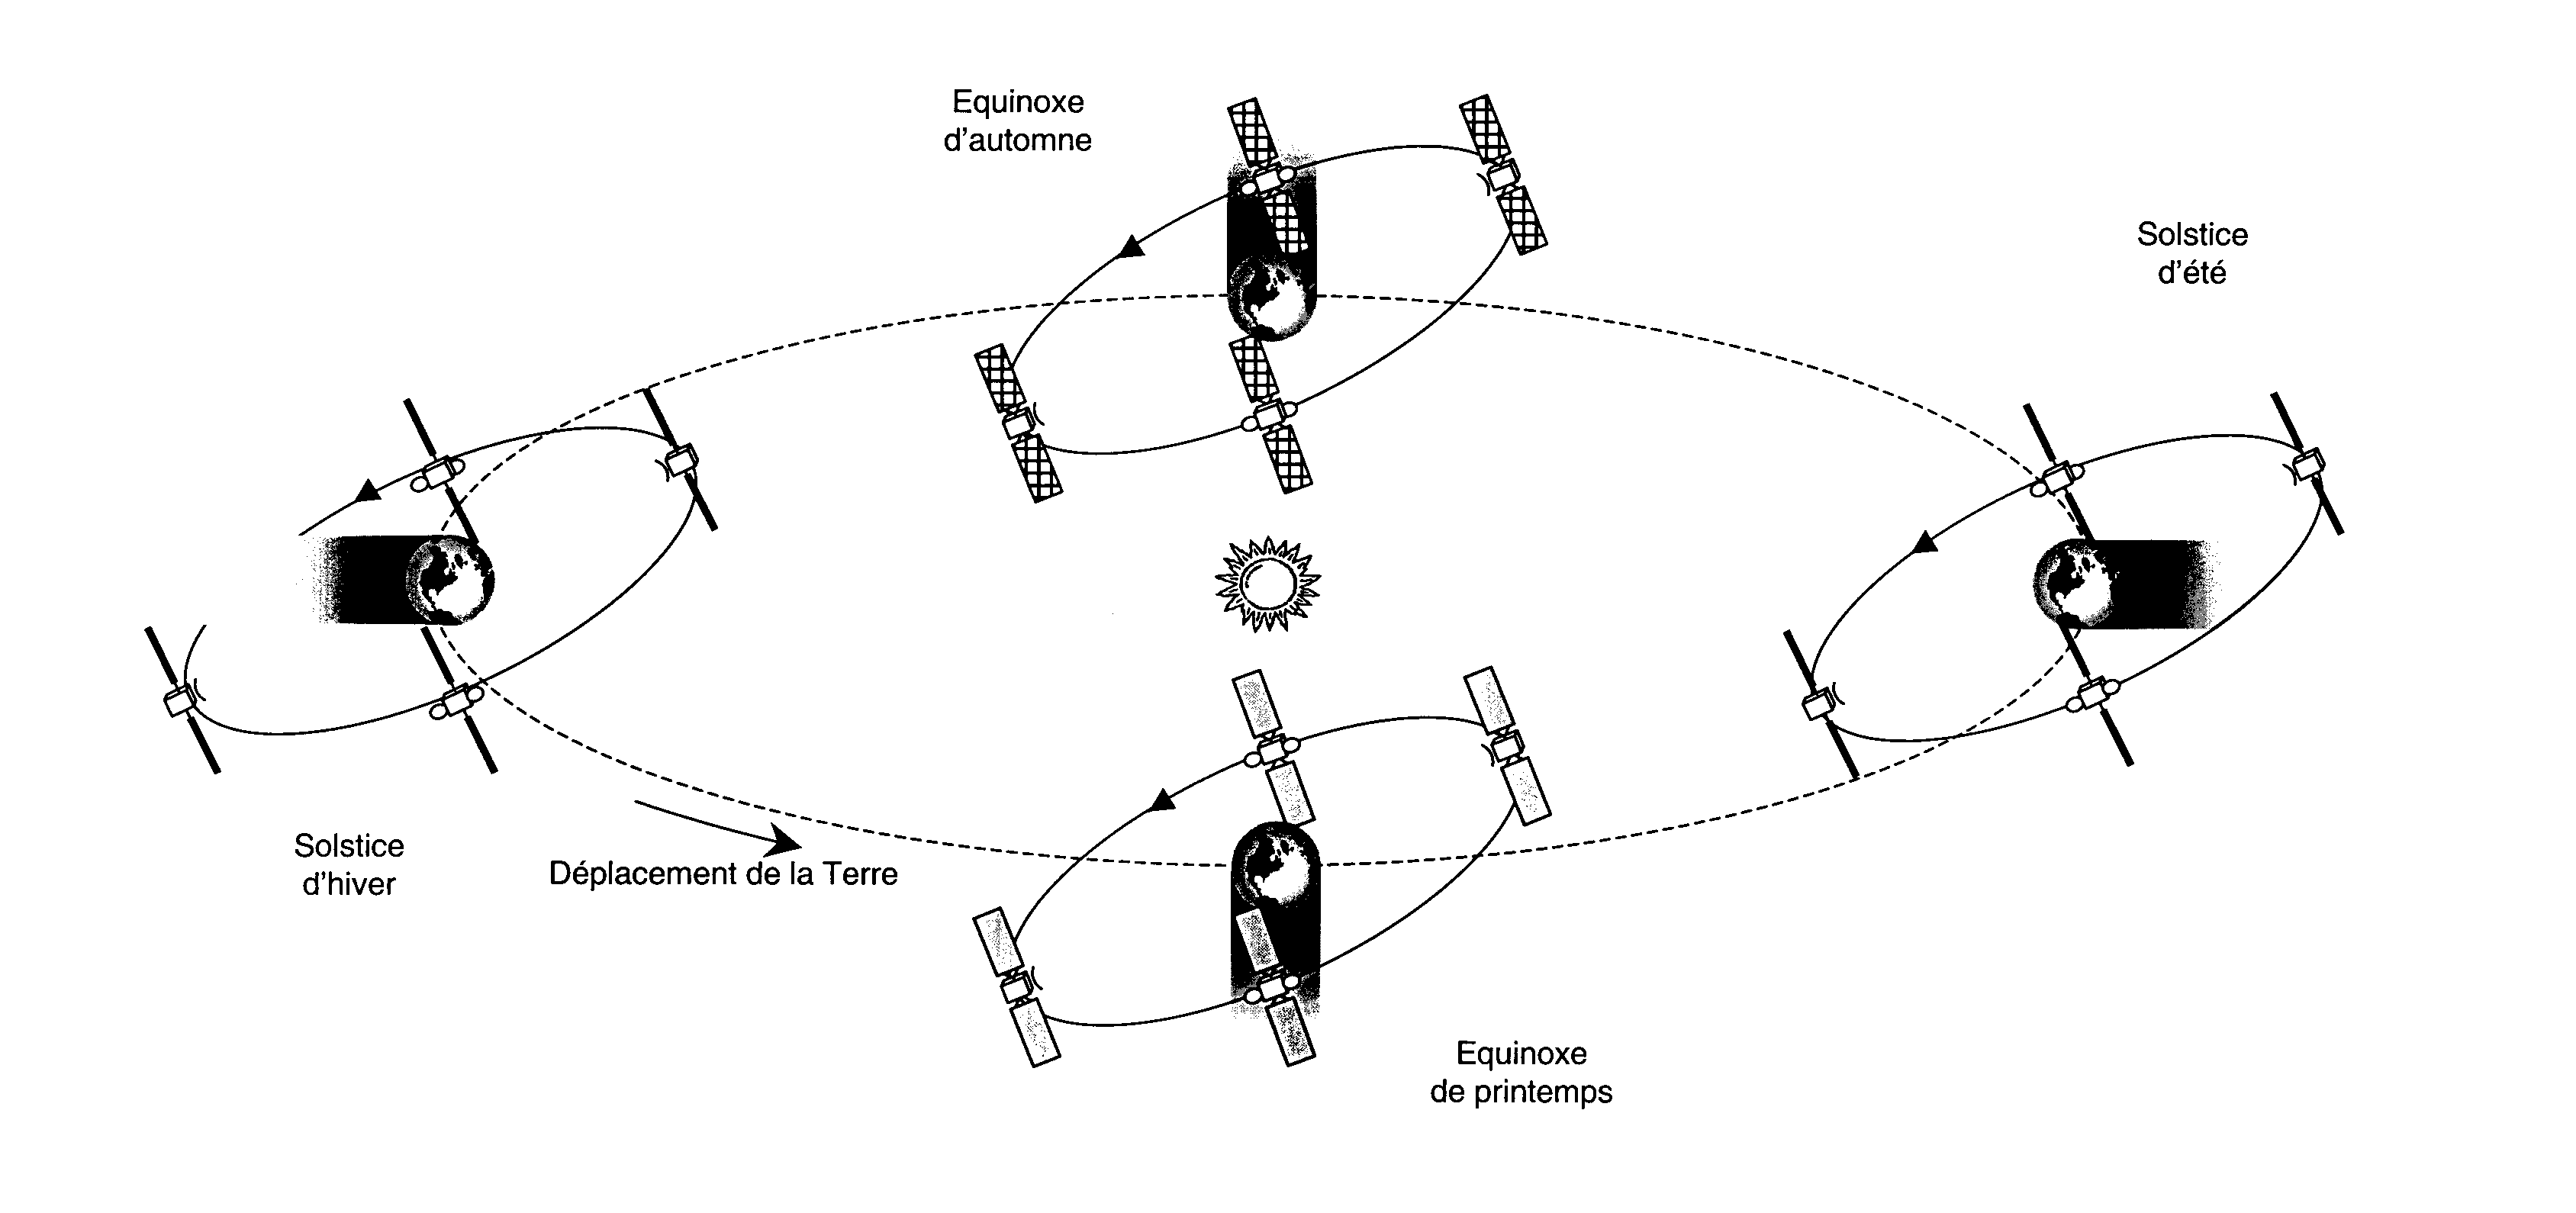
\includegraphics[width=0.65\textwidth]{fig/orbit.png}
  \caption{Title}
  \label{fig:orbit}
\end{figure}

\begin{table}[t]
    \begin{center}
        \caption{Title}
        \label{tab:numbers}

        \begin{tabular}{ |c|c|c|c| } 
         \hline
        \multirow{2}{*}{\textbf{First}} & \multicolumn{3}{c|}{\textbf{Second}}\\ \cline{2-4}
                                        &  \textbf{-1} & \textbf{0} & \textbf{1}\\ \hline
        A	                            &   212        &	343     &	7567\\ \hline
        B	                            &   133	       &    24234   &	567 \\ \hline
        C	                            &   6545       &	34234	&   796 \\ \hline
        D                               &	546        &	34244   &   879 \\ \hline
        \end{tabular}
    \end{center}
\end{table}

\subsection{Abbreviations and Acronyms}

Define abbreviations and acronyms the first time they are used in text, even after they have been defined in the abstract. Abbreviations such as TTC, TM, TC, ac and dc do not have to be defined. Do not use abbreviations in the title.

\section{ADDING CITATIONS}

Number citations consecutively in square brackets \cite{johnson1988space}. Refer simply to the reference number, as in \cite{grun1985collisional}. Do not use ``Ref. \cite{grun1985collisional}'' or ``reference \cite{grun1985collisional}” except at the beginning of a sentence: ``Reference \cite{grun1985collisional} was the first...'' The title of the book or of the journal shall be in italic script. See the section below.

\bibliographystyle{esacit}
\bibliography{references}

\end{document}
